\documentclass[border=5pt]{standalone}
\usepackage{fontspec}
\usepackage{unicode-math}
\setmainfont{Noto Serif}
\setmathfont{STIXTwoMath-Regular.otf}
\usepackage{tikz}
\usetikzlibrary{arrows.meta,calc,decorations.pathmorphing,decorations.markings}
\tikzset{
 level/.style={draw=black,line width=.62pt,line cap=butt},
 axis/.style={draw=black,line width=.72pt,-{Latex[length=2.2mm,width=1.35mm]}},
 pump/.style={draw=black,line width=.8pt,-{Latex[length=2.4mm,width=1.5mm]}},
 curve/.style={draw=black,line width=1.35pt,line cap=round,line join=round},
 label/.style={font=\fontsize{14}{17}\selectfont,inner sep=2pt},
 link/.style={draw=black,line width=.8pt,line cap=round,line join=round},
 waveline/.style={link,decorate,decoration={snake,amplitude=.24mm,segment length=2.6mm,pre length=0mm,post length=0mm}}
}
\pagestyle{empty}
\begin{document}
% Figure 11.1. Four zones, repeated upward photon steps.
% Distribution is schematic, not a fit to measurements; smooth Gaussian
% is used only for the qualitative envelope. Parameters have no physical units.
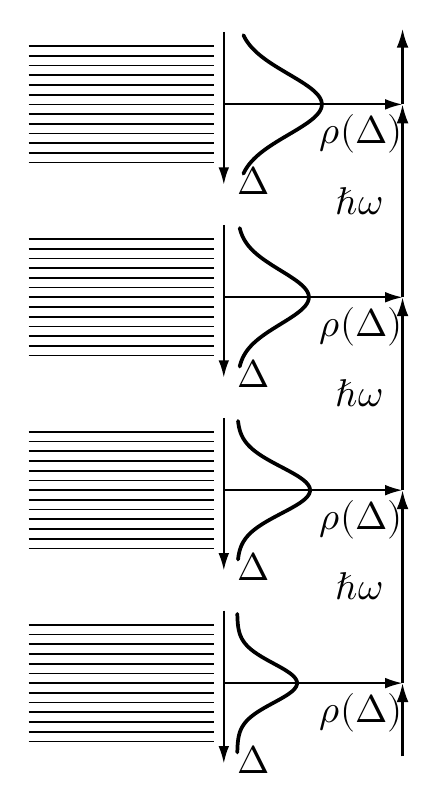
\begin{tikzpicture}[x=1cm,y=1cm]
\def\ZoneSpacing{2.45}
\def\ProfileWidth{1.02} % base only; local parameters below
\def\ProfileSigma{0.31} % base only; local parameters below
\def\ZoneHalf{0.74}
\foreach \i in {0,1,2,3}{
 \pgfmathsetmacro{\cy}{0.95+\i*\ZoneSpacing}
 \pgfmathsetmacro{\ThisProfileWidth}{.76+.075*\i+.09*mod(\i,2)}
 \pgfmathsetmacro{\ThisSigma}{.25+.045*\i}
 \coordinate (centre\i) at (2.65,\cy);
 \coordinate (pump\i) at (4.75,\cy);
 \foreach \j in {0,...,12}{
  \pgfmathsetmacro{\yy}{\cy-\ZoneHalf+2*\ZoneHalf*\j/12}
  \draw[level] (0,\yy) -- (2.35,\yy);
 }
 \draw[axis] (2.48,{\cy+0.92}) -- (2.48,{\cy-1.02});
 \node[label,anchor=west] at (2.58,{\cy-.97}) {$\Delta$};
 \draw[axis] (2.48,\cy) -- (pump\i);
 \draw[curve,variable=\s,domain=-.88:.88,samples=180]
   plot ({2.65+\ThisProfileWidth*exp(-.5*(\s/\ThisSigma)^2)},{\cy+\s});
 \node[label,anchor=north west] at (3.62,{\cy-.05}) {$\rho(\Delta)$};
}
% One continuous pump axis, with upward tips at the centres of the zones.
\draw[pump] (4.75,0.02) -- (pump0);
\foreach \i in {0,1,2}{
 \pgfmathtruncatemacro{\j}{\i+1}
 \draw[pump] (pump\i) -- (pump\j);
 \node[label,anchor=east] at (4.57,{0.95+(\i+.5)*\ZoneSpacing}) {$\hbar\omega$};
}
\draw[pump] (pump3) -- (4.75,9.26);
\end{tikzpicture}
\end{document}
